\documentclass[10pt,conference,compsocconf]{IEEEtran}

\usepackage{hyperref}
\usepackage{graphicx}
\usepackage{amsmath}
\usepackage{amssymb}
\usepackage[table]{xcolor}
\definecolor{tabhighlight}{rgb}{0.9, 0.97, 0.9}
\usepackage{booktabs}
\usepackage{tikz}
\usetikzlibrary{arrows.meta,positioning}

\begin{document}
\title{Test-Time Compositional Control for Diffusion Models}

\author{
  Yunyi Chen (423371), Xinran Wang (416485), Shengze Jiang (386685), Hantao Zhang (405442)\\
  \textit{CS-503 Project Progress Report}
}

\maketitle

\section{Milestone Progress}

Our proposal studies training-free compositional control for diffusion models: satisfying multiple test-time constraints, such as different left/right semantic prompts and a coherent transition between them.
It is motivated by latent diffusion models~\cite{rombach2022high}, classifier-free guidance, DiffCollage-style factor composition~\cite{zhang2023diffcollage}, and recent correction-based views of biased composition~\cite{skreta2024superposition,skreta2025fkc}. To further instantiate the "bridge variable" — defined here as the overlapping intermediate patches in panoramic image generation — this milestone focused on making the bridge formulation executable in a Stable Diffusion text-prompt experiment.



\subsection{Clarified Problem Setting}

We make the bridge variable concrete as the image overlap shared by adjacent diffusion factors, rather than treating $y$ as an unspecified latent state.
For neighboring factors $p(x,y)$ and $p(y,z)$, the sampler should compose their predictions without double-counting the shared overlap $y$ while correcting local inconsistencies.

\subsection{Method Details}

Figure~\ref{fig:method-pipeline} summarizes our current text-prompt bridge pipeline, which uses frozen Stable Diffusion 1.5 components: the CLIP text encoder, UNet denoiser, VAE decoder, and DDIM scheduler.
All methods share the same prompts, seed, denoising steps, guidance scale, window size, and overlap size, and differ only in how per-window noise predictions are composed.

\begin{figure}[h]
\centering
\resizebox{\linewidth}{!}{
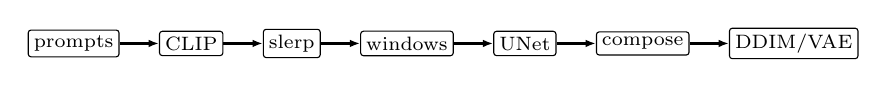
\begin{tikzpicture}[
node distance=5mm,
box/.style={draw, rounded corners=1pt, align=center, font=\scriptsize, inner sep=2pt},
arrow/.style={-{Latex[length=1.3mm]}, thick}
]
\node[box] (p) {prompts};
\node[box, right=of p] (c) {CLIP};
\node[box, right=of c] (s) {slerp};
\node[box, right=of s] (w) {windows};
\node[box, right=of w] (u) {UNet};
\node[box, right=of u] (m) {compose};
\node[box, right=of m] (d) {DDIM/VAE};
\draw[arrow] (p)--(c);
\draw[arrow] (c)--(s);
\draw[arrow] (s)--(w);
\draw[arrow] (w)--(u);
\draw[arrow] (u)--(m);
\draw[arrow] (m)--(d);
\end{tikzpicture}}
\caption{Compact pipeline for the current text-prompt bridge experiment.}
\label{fig:method-pipeline}
\vspace{-2mm}
\end{figure}


Let $u_t\in\mathbb{R}^{4\times64\times W}$ be the noisy latent of the whole generated image at timestep $t$.
We split it into $N$ overlapping latent windows
\begin{equation}
    w_i(u_t) = u_t[:, :, a_i:b_i], \qquad i=1,\ldots,N,
\end{equation}
where each window has width 64 latent pixels and neighboring windows overlap by 32 latent pixels.
If $e_L$ and $e_R$ are the CLIP text embeddings of the left and right prompts, the condition for window $i$ is obtained by spherical interpolation,
\begin{equation}
    e_i = \mathrm{slerp}\!\left(e_L,e_R,\alpha_i\right),\qquad
\alpha_i=\frac{i-1}{N-1}.
\end{equation}
Thus the left window is guided by the left prompt, the right window is guided by the right prompt, and middle windows receive intermediate semantic conditions.

For each window, Stable Diffusion gives a classifier-free-guided noise prediction
\begin{equation}
\epsilon_i = \epsilon_\theta(w_i,t,\emptyset) + \gamma\left[ \epsilon_\theta(w_i,t,e_i)-\epsilon_\theta(w_i,t,\emptyset) \right],
\end{equation}
where $\gamma$ is the guidance scale.
The remaining question is how to compose the window-level predictions into one full-latent prediction
$\epsilon_{\mathrm{full}}(u_t,t)$.

\textbf{DiffCollage-style implicit marginal subtraction.} The factor-graph view corrects the double counting by subtracting an overlap marginal.
The ideal distributional expression is
\begin{equation}
p_{\mathrm{fg}}(x,y,z) \propto \frac{p(x,y)p(y,z)}{p(y)} .
\end{equation}
In score form, this becomes
\begin{equation}
s_{\mathrm{fg}} = s_{xy}\oplus s_{yz} - s_y ,
\end{equation}
where $s_y=\nabla_y\log p(y)$.
Our derivation points out that the marginal score can be estimated implicitly from the joint score:
\begin{equation}
\nabla_y\log p(y) = \mathbb{E}_{x\mid y} \left[\nabla_y\log p(x,y)\right].
\end{equation}
In our Stable Diffusion implementation, we instantiate this by running the model on the overlap region itself and subtracting the corresponding overlap noise prediction before merging:
\begin{equation}
\epsilon_{\mathrm{dc}} = \mathrm{Merge} \left(\epsilon_1,\ldots,\epsilon_N;\, -\epsilon_{\mathrm{overlap},1},\ldots, -\epsilon_{\mathrm{overlap},N-1}\right).
\end{equation}
Each overlap marginal uses the same interpolated prompt embedding as its parent window, so the subtraction is semantically aligned with the local text condition.

\textbf{Naive composition.} The naive baseline directly averages overlapping window predictions:
\begin{equation}
\epsilon_{\mathrm{naive}}(u_t,t) = \mathrm{Merge}\left(\epsilon_1,\ldots,\epsilon_N\right).
\end{equation}
This is analogous to multiplying local pairwise components without removing the overlap bias.
In the three-variable notation, it corresponds to using
$p(x,y)p(y,z)$ while the shared variable $y$ is counted twice.

\textbf{Bridge correction (Ours).} The theoretical correction in our derivation introduces a coupling factor
\begin{equation}
R(x,y,z) = \frac{p(x,z\mid y)} {p(x\mid y)p(z\mid y)}
\end{equation}
and therefore a corrected score
\begin{equation}
s_{\mathrm{bridge}} = s_{xy}\oplus s_{yz} - s_{y,\mathrm{implicit}} + \nabla\log R(x,y,z).
\end{equation}
The role of $R$ is to measure the residual dependence between the two sides after conditioning on the bridge variable.
If $x$ and $z$ were conditionally independent given $y$, then $R=1$ and the DiffCollage-style term would be sufficient.
When the two sides still need to coordinate through the bridge, $\nabla\log R$ should push the two local predictions toward a globally consistent transition.

The current experiment implements a conservative proxy for this correction.
After computing the DiffCollage-style composed prediction, we convert each window's noise prediction to a Tweedie/DDIM estimate of the clean latent~\cite{song2022denoisingdiffusionimplicitmodels}:
\begin{equation}
\hat{x}_{0,i} = \frac{w_i(u_t)-\sqrt{1-\bar{\alpha}_t}\,\epsilon_i} {\sqrt{\bar{\alpha}_t}} .
\end{equation}
For neighboring windows, we compute the mismatch between the two predicted clean overlaps:
\begin{equation}
r_i = \hat{x}_{0,i}^{\mathrm{right}} - \hat{x}_{0,i+1}^{\mathrm{left}} .
\end{equation}
The correction adds opposite forces to the two sides of the shared overlap,
\begin{equation}
\Delta\epsilon_i^{\mathrm{right}} \mathrel{+}=
    \lambda_t r_i,\qquad
\Delta\epsilon_{i+1}^{\mathrm{left}} \mathrel{-}= \lambda_t r_i,
\end{equation}
with
\begin{equation}
\lambda_t = \frac{\lambda}{\sqrt{\bar{\alpha}_t}},
\end{equation}
followed by clipping for numerical stability.
The full prediction is
\begin{equation}
\epsilon_{\mathrm{bridge}} = \epsilon_{\mathrm{dc}} + \Delta\epsilon .
\end{equation}
This is not a closed-form estimator of $\nabla\log R$, but it follows the same principle: use denoised overlap disagreement as a signal that the two pairwise experts are not globally consistent.
Thus, the current Stable Diffusion experiment implements a correction-based approximation, while the fully direct $P(x,y)P(y,z)$ composition without an explicit tree-style marginal remains a final target.

\subsection{Progress and Results}

\textbf{Scope of the First Milestone:} We build directly on DiffCollage under the conditional-independence assumption $R \equiv 1$, where the exact factorization
\begin{align}
p(x,y,z) &= \underbrace{\frac{p(x,y)\cdot p(y,z)}{p(y)}}_{p_{\text{DC}}} \cdot R(x,y,z), \label{eq:joint-decomp} \\
R &:= \frac{p(x,z\mid y)}{p(x\mid y)\cdot p(z\mid y)}
\end{align}
shows that $p_{\text{DC}}$ is the projection of the true joint onto $R\equiv 1$. Our $\Delta\epsilon$ corrector enforces overlap consistency in this regime via a Tweedie-based proxy in $\hat{x}_0$ space---without estimating $R \neq 1$ as in SuperDiff~\cite{skreta2024superposition} or FK Correctors~\cite{skreta2025fkc}. Based on pre-milestone factor-graph tests, we scope this milestone to a text-prompt bridge prototype, deferring a principled $R \neq 1$ treatment to later stages.

We ran 22 prompt pairs spanning nature, weather, seasons, day/night, urban, and abstract transitions.
Table~\ref{tab:text-results} reports the text-prompt bridge comparison under the shared evaluation protocol. Figure~\ref{fig:three-method-examples} shows a qualitative comparison of the three composition strategies.
Seam MSE is computed between narrow pixel strips around each visible window boundary, so it measures local smoothness rather than prompt satisfaction or overall quality.

\begin{table}[h]
\centering
\caption{Text-prompt bridge sweep over 22 prompt pairs.}
\label{tab:text-results}
\begin{tabular}{lccc}
\toprule
Method & Samples & Seam MSE $\downarrow$ & Seam Max $\downarrow$ \\
\midrule
DiffCollage & 22 & 0.0307 & 0.0367 \\
Naive & 22 & 0.0248 & 0.0302 \\
\rowcolor{tabhighlight}
Ours $c=0.01$ & 22 & 0.0185 & 0.0224 \\
\bottomrule
\end{tabular}
\end{table}

\begin{figure}[h]
\centering
\begin{minipage}{0.32\linewidth}
\centering
\includegraphics[width=\linewidth]{\detokenize{./figures/__a_foggy_morning_valley_a_bright_sunny_afternoon/diffcollage_DEGRADED/a_foggy_morning_valley_to_a_bright_sunny_afternoon/sample_000.png}}
\scriptsize DiffCollage
\end{minipage}
\hfill
\begin{minipage}{0.32\linewidth}
\centering
\includegraphics[width=\linewidth]{\detokenize{./figures/__a_foggy_morning_valley_a_bright_sunny_afternoon/naive_DEGRADED/a_foggy_morning_valley_to_a_bright_sunny_afternoon/sample_000.png}}
\scriptsize Naive
\end{minipage}
\hfill
\begin{minipage}{0.32\linewidth}
\centering
\includegraphics[width=\linewidth]{\detokenize{./figures/__a_foggy_morning_valley_a_bright_sunny_afternoon/proposal_c0.01/a_foggy_morning_valley_to_a_bright_sunny_afternoon/sample_000.png}}
\scriptsize Ours
\end{minipage}
\caption{Prompt pair `a foggy morning valley' to `a bright sunny afternoon'.}
\label{fig:three-method-examples}
\vspace{-2mm}
\end{figure}

These results are encouraging because the proposal correction gives the lowest seam MSE in the current text-prompt setting, while producing more natural prompt-conditioned transitions between the two endpoint prompts.

\section{Discussion \& Next Steps}

The main progress is that the original bridge-variable idea is now an executable Stable Diffusion text-prompt composition framework.
What remains unresolved is whether lower seam error also means better prompt satisfaction and global coherence.
The current $\hat{x}_0$ correction is still heuristic and not a full estimator of $\nabla\log R$.

Until the next report, we will:
\begin{itemize}
\item add perceptual or quality metrics so seam MSE is not the only signal;
\item ablate CFG variants, correction strength, clipping, and timestep scheduling;
\item connect the bridge prototype back to the original content/style image-editing goal.
\end{itemize}

For the final project, our goal is to present the bridge formulation as a training-free text-prompt composition method.

\section{Author Contribution Statement}

Hantao Zhang developed the bridge-correction theoretical formalism.
Yunyi Chen and Shengze Jiang implemented the bridge-worker framework.
Xinran Wang contributed to evaluation design and metric discussion.
All authors discussed the experimental deviations from the initial proposal and contributed to this progress report.

\[
\epsilon_{\mathrm{PoE}}=\mathrm{Merge}(\epsilon_1,\ldots,\epsilon_N)
\]

\[
G_t^k=\frac{1}{D}\sum_i \left\langle \epsilon_{i,R}^{k}(t),\,\epsilon_{i+1,L}^{k}(t)\right\rangle
\]

\[
\log w_t^k=\log w_{t+1}^k+\beta G_t^k
\]

\[
z_0^{*}=z_0^{\arg\max_k \log w_0^k}
\]

\[
k^{*}=\arg\max_k \log w_0^k,\qquad z_0^{*}=z_0^{k^{*}}
\]

\bibliographystyle{IEEEtran}
\bibliography{cs503_style_literature}

\end{document}
